\chapter{The $\plonk$ protocol}
\label{chap:3}

With the knowledge from the previous chapter, we can get to the description of the protocol itself. $\plonk$ protocol has a trusted setup in the form of the \textit{structured reference string} $SRS$ that can be reused for proofs on multiple circuits. The natural benefit is that the setup parameters could be used indefinitely, enabling $\plonk$ to be a multi-party protocol. This fundamental property makes the protocol valuable and promising for application in blockchain technologies. It is essential to mention that the security is based on the hardness of the discrete logarithm problem on elliptic curves. The original paper uses KZG \cite{KZG} (Kate, Zaverucha, Goldberg) commitments, but the protocol could be altered to use another polynomial commitment scheme. These commitments have constant size. 

\begin{table}[h]
    \centering
    \resizebox{\textwidth}{!}{
        \begin{tabular}{ c | c c c c}
            protocol & proof size & public parameters & verifier time & trusted setup \\ 
            \hline
            Groth16      & $\bigO{1}$             & $\bigO{|C|}$ & $\bigO{1}$           & per circuit \\ 
            Plonk & $\bigO{1}$         & $\bigO{|C|}$ & $\bigO{1}$           & universal \\ 
            Bulletproofs & $\bigO{\log{|C|}}$   & $\bigO{1}$   & $\bigO{|C|}$        & no\\ 
            STARK        & $\bigO{\log^2{|C|}}$  & $\bigO{1}$   & $\bigO{\log{|C|}}$  & no \\ 
            DARK         & $\bigO{\log{|C|}}$     & $\bigO{1}$   & $\bigO{\log{|C|}}$               & no \\ 
        \end{tabular}
    }
    \caption{Comparison of protocols}
\end{table}

The table above presented on Dan Boneh's lecture \cite{Boneh2024} compares the $\plonk$ protocol against other protocols. The big benefit is that the protocol has a constant size of the proof composed of 9 polynomial commitments and 6 polynomial openings. The public parameter SRS is directly proportional to the size of the proof, as we will show in \Cref{sec:verification}. The trusted setup is universal in the sense that the public parameter can be used for any circuit of a given bound on the number of gates. 

Besides the trusted one-time setup, the protocol has a setup phase for computing common preprocessed input for a circuit. The rest of the prover protocol is split into five rounds. Finally, there is an algorithm for the verifier, but we will not get into the details since the verifier implicitly checks all parts of the proof. The whole protocol is one batched KZG polynomial scheme that proves multiple evaluations on multiple points. So the verifier algorithm does some trivial validity checks to verify that elements of the correct field and groups were provided, then reconstructs proof fragments and finally does batch verification. The simplified protocol is shown in the diagram below. In the next chapter, we will show a complete prover algorithm diagram. 

\begin{figure}[ht]
    \centering
    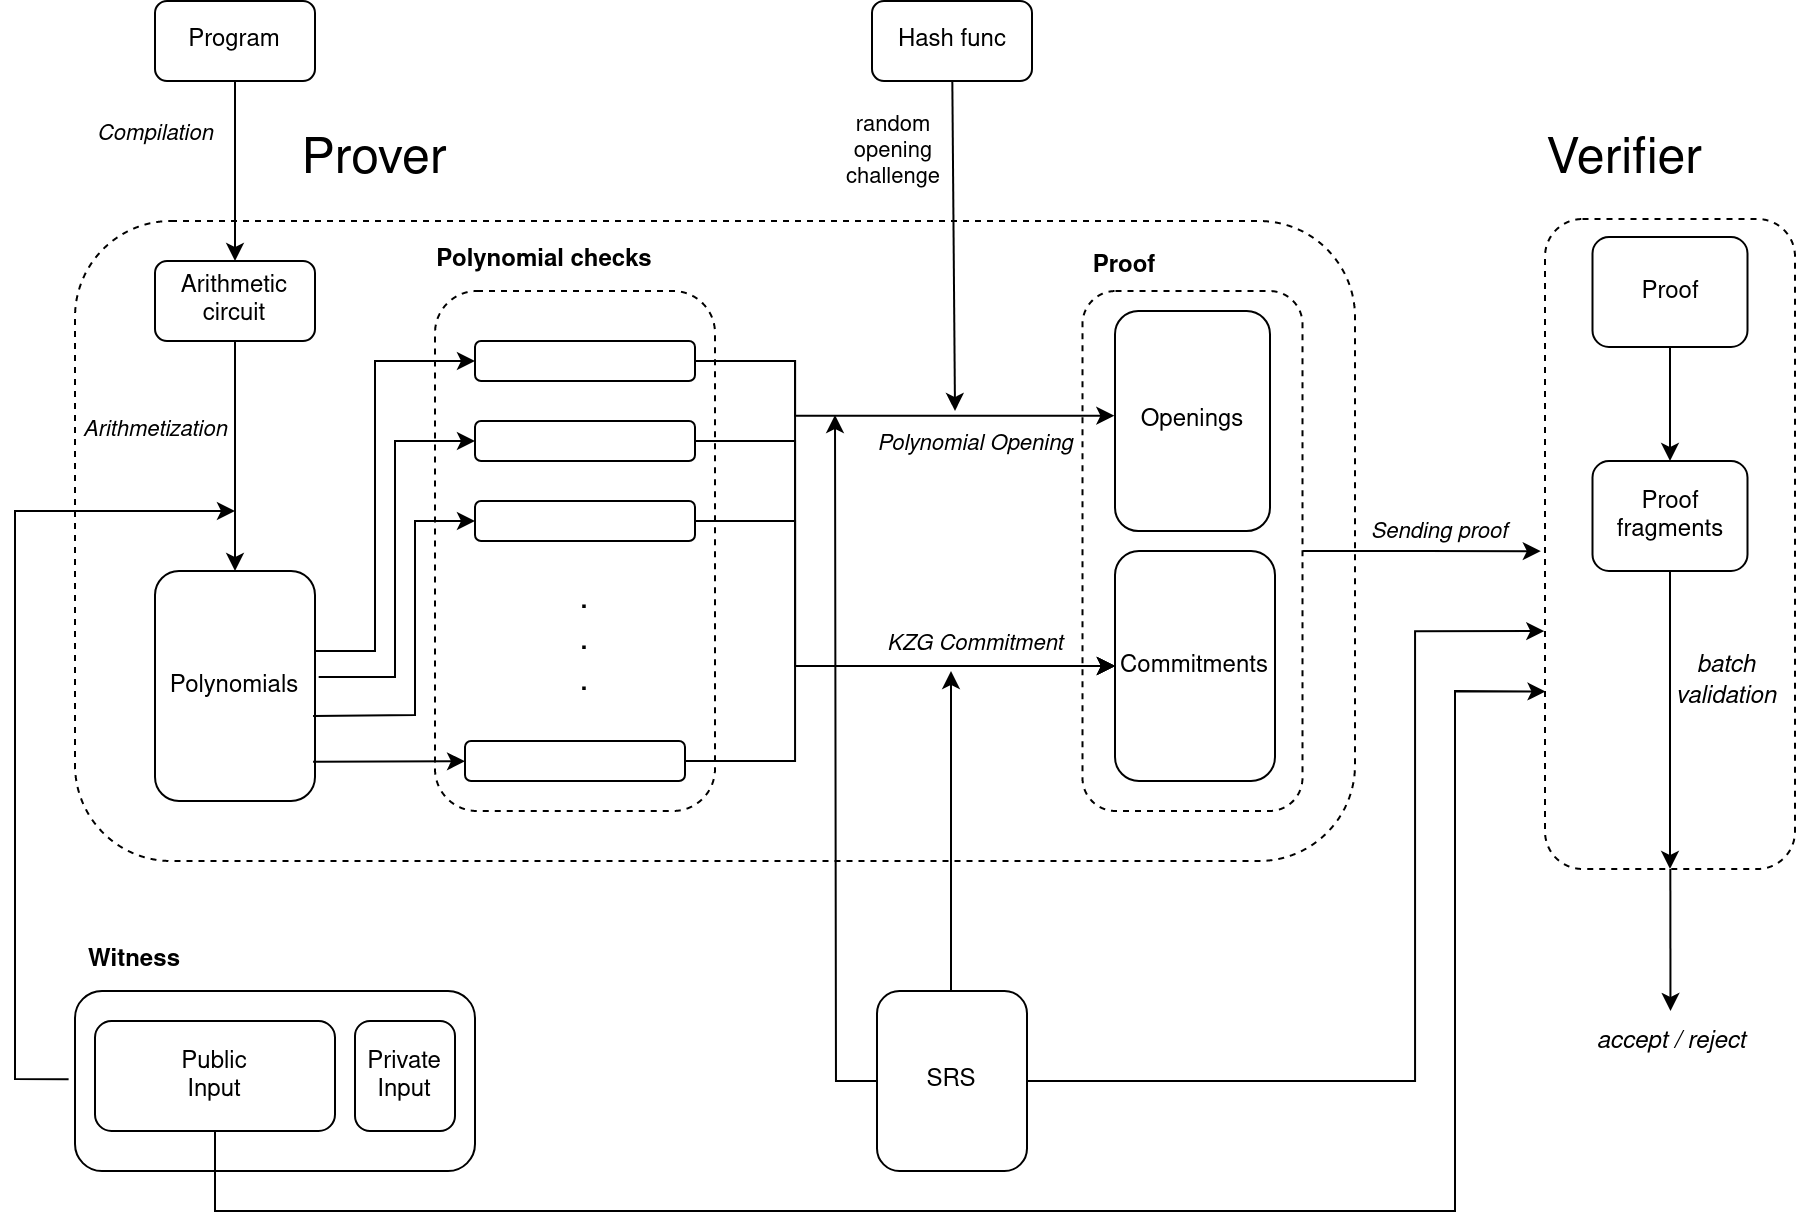
\includegraphics[width=1\linewidth]{round-figures/round1/plonk_better_overview.drawio.png}
    \caption{Simplified protocol}
\end{figure}

% Diagrams provided in this chapter have the following legend:
% A diagram will be provided to show how the protocol works. Below is the legend for these diagrams.
% \begin{figure}[H]
%     \centering
%     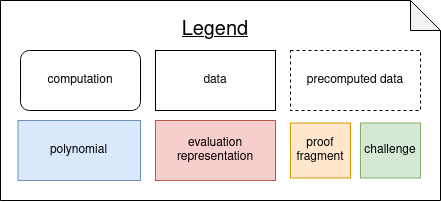
\includegraphics[width=0.5\linewidth]{round-figures/legend.drawio.png}
%     \caption{Legend for the Plonk diagrams}
% \end{figure}


% ==============================================================================
% ===SETUP======================================================================
% ==============================================================================
\section{Setup algorithm}
\label{chap:round0}
The setup algorithm describes the calculation of the common pre-processed input. It is not considered a routine protocol round. The only trusted part is the public key \textit{structured reference string} $SRS$ that is not tied to the structure of an arithmetic circuit but to the upper bound of the number of the circuit gates. This means the preprocessed setup can be updated for new circuits while the $SRS$ can be reused. As mentioned earlier, the $SRS$ cannot be generated by the prover because discovering the generation key $\tau$ would allow one to forge commitments and, therefore, invalidate the whole protocol.

\subsection{Public Information }
Since the $\plonk$ protocol runs KZG, all of the parties should have access to the information needed in KZG polynomial commitment scheme $$(\field, \mathbb{G}_1, \mathbb{G}_2, \mathbb{G}_t, e, G_1, G_2, G_t, SRS)$$ To revise $\field$ is a prime field, $(\mathbb{G}_1, \mathbb{G}_2, \mathbb{G}_t)$ are groups of points on elliptic curves and $e$ is efficiently computable group pairing $e: \mathbb{G}_1 \times \mathbb{G}_2 \rightarrow \mathbb{G}_t$. Lastly $G_1, G_2$ are group generators of $\mathbb{G}_1, \mathbb{G}_2$. Moreover, there needs to be a KZG setup ceremony generating the \textit{structured reference string} SRS, which is public. 

\subsection{Preprocessed Input}
Below is summed up the common preprocessed input that is available to both parties. Each of the components will be described in detail in the following rounds.

\begin{itemize}
    \item $n$ number of gates in the arithmetic circuit
    \item $k_1, k_2 \in \field$ are needed to create $k_1 H , k_2 H$ such that the union $H' = H \cup k_1 H \cup k_2H)$ contains $3n$ distinct elements. This will be further explained in the \hyperref[chap:round2]{round 2}.
    \item permutation function: $\sigma^*: [3n] \rightarrow H'$ which is rotation of equivalence classes in the witness $w$ as described in \hyperref[sec:wiring-check]{wiring check}
    \item selector polynomials: $q_m(x), q_l(x), q_r(x), q_o(x), q_c(x)$ interpolated from selector vectors $q_m, q_l, q_r, q_o, q_c$ introduced in \hyperref[chap:arithmetization]{arithmetization}

    % \begin{align*}
    %     q_m(x) = \sum_{i=1}^n L_i(x) q_{m_i} \\
    %     q_l(x) = \sum_{i=1}^n L_i(x) q_{l_i} \\
    %     q_r(x) = \sum_{i=1}^n L_i(x) q_{r_i} \\
    %     q_o(x) = \sum_{i=1}^n L_i(x) q_{o_i} \\
    %     q_c(x) = \sum_{i=1}^n L_i(x) q_{c_i} \\
    % \end{align*}

    \begin{equation*}
        \begin{array}{cc}
        q_m(x) = \sum_{i=1}^n L_i(x) q_{m_i} & q_o(x) = \sum_{i=1}^n L_i(x) q_{o_i} \\
        q_l(x) = \sum_{i=1}^n L_i(x) q_{l_i} & q_c(x) = \sum_{i=1}^n L_i(x) q_{c_i} \\
        q_r(x) = \sum_{i=1}^n L_i(x) q_{r_i} 
        \end{array}
    \end{equation*}
        
    \item permutation polynomials: $S_{\sigma_1}, S_{\sigma_2}, S_{\sigma_3}: [n] \rightarrow H'$ interpolated from $\sigma^*$
    
    \begin{equation*}
        \begin{array}{cc}
        S_{\sigma_1}(x) = \sum_{i=1}^n L_i(x) \sigma^*(i) & S_{\sigma_2}(x) = \sum_{i=1}^n L_i(x) \sigma^*(n+i) \\
        S_{\sigma_3}(x) = \sum_{i=1}^n L_i(x) \sigma^*(2n+i)
        \end{array}
    \end{equation*}
\end{itemize}


% ==============================================================================
% ===ROUND1=====================================================================
% ==============================================================================
\section{Round 1}
\label{chap:round1}

% \begin{figure}[H]
%     \label{fig:round1}
%     \centering
%     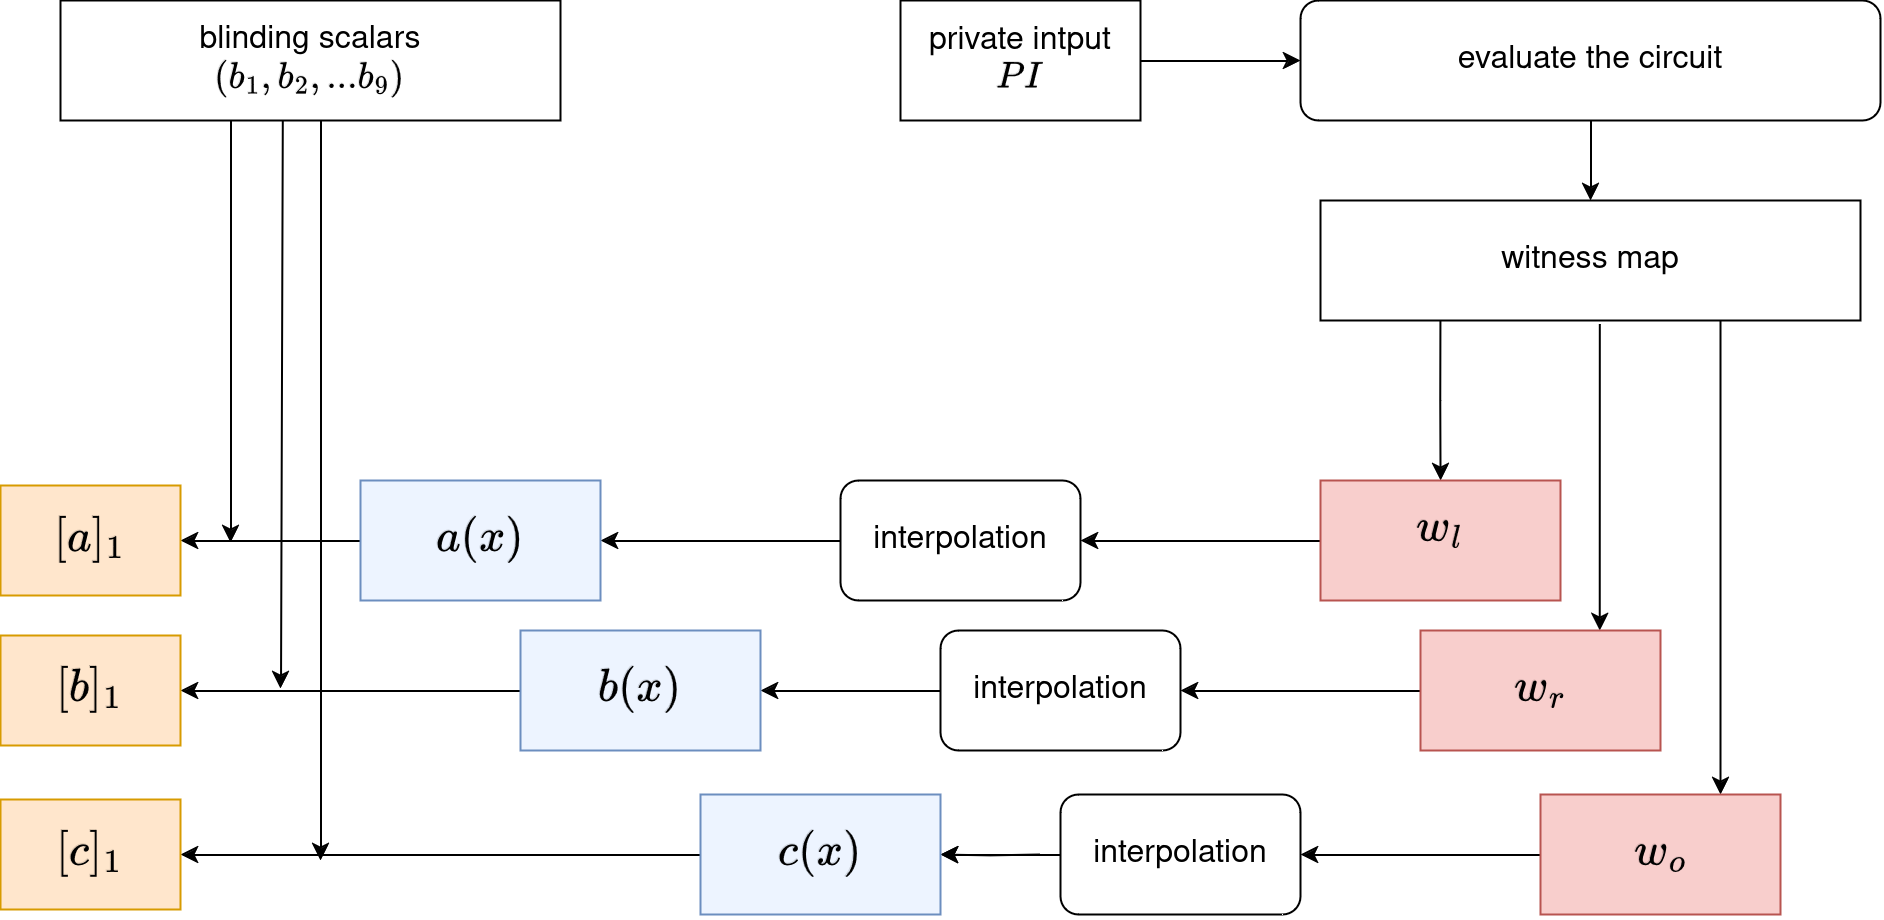
\includegraphics[width=1\linewidth]{round-figures/round1/round1.drawio.png}
%     \caption{Round 1 Diagram}
% \end{figure}

\subsection{Computing wire polynomials}

The proof generation starts by computing the wire polynomials and committing to them. Recall that we get the witness values in the arithmetization as columns of the computational table. The domain is chosen as $H = \{1, \omega, \omega^2, \ldots, \omega^{n-1}\}$ where $\omega^n = 1$. Choosing such a domain allows for a sparse representation of the vanishing polynomial as $Z_H(x) = x^n -1$.

By pairing this domain with the witness $w$, we get the wire polynomials in the evaluation domain. To make commitments, the polynomial needs to be in the coefficient form to evaluate it at the point $\tau$. Conversion to the coefficient form can be achieved by applying the Lagrange interpolation.

Finally, they should be blinded to ensure that the commitment to the wire polynomials does not leak information about the wire polynomial. As described in \Cref{theorem:blinding}, this construction maintains the zero-knowledge property. The prover must uniformly randomly sample 9 blinding scalars $(b_1, b_2, \ldots, b_9)$. In round 1, there are nine sampled blinding scalars, even though we only need 6. The remaining will be used in the following rounds.

\procedureblock[linenumbering]{$Round1_{\prover}$}{
    (b_1, \ldots, b_9) \gets \field^9 \\
    a(x) = (b_1x + b_2)Z_H(x) + \sum_{i=0}^{n-1} w_i L_i(x) \\
    b(x) = (b_3x + b_4)Z_H(x) + \sum_{i=0}^{n-1} w_{n+i} L_i(x) \\
    c(x) = (b_5x + b_6)Z_H(x) + \sum_{i=0}^{n-1} w_{2n+i} L_i(x) \\
    \pcreturn [a]_1, [b]_1, [c]_1
}

% ==============================================================================
% ===ROUND2=====================================================================
% ==============================================================================
\section{Round 2}
\label{chap:round2}

This round ensures the circuit's copy constraints. We will start by showing that constraints hold for inter-vector checks and then extend them to intra-vector checks.

% \begin{figure}[H]
%     \centering
%     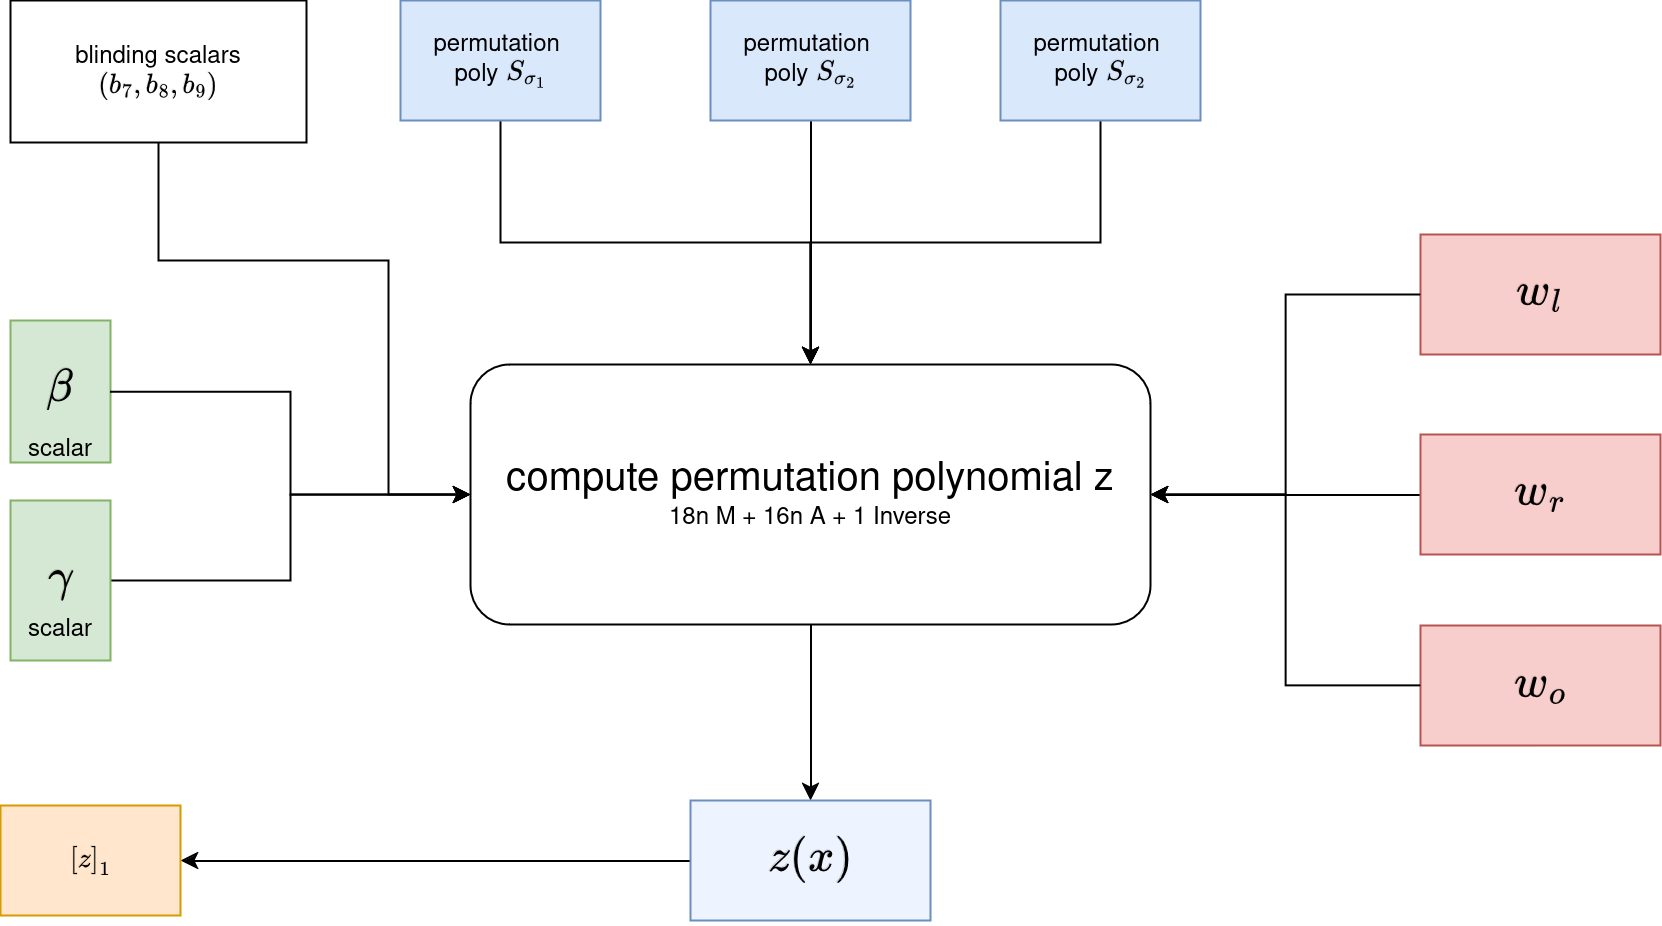
\includegraphics[width=1\linewidth]{round-figures/round2/round2.drawio.png}
%     \caption{Round 2 Diagram}
%     \label{fig:round2}
% \end{figure}


\section{Permutation check}
\label{permutation-check}
Let's say that an enemy gives you two vectors $p = [p_1, p_2 \ldots p_n], q = [q_1, q_2 \ldots q_n]$ and you need to decide if they are permutations of each other. So we check if there is a $\sigma$ such that $\forall i \in [n] \exists j \in [n]: \sigma(p_i) = q_j$. You could compare elements one by one, but that is too slow. There is a smarter way smarter way to do this. A good start is to contract the vectors into a single value. So, we can perform, for example, something like a product check where we compare:$$p_1 \cdot p_2 \ldots \cdot p_n \stackrel{?}{=} \sigma(q_1) \cdot \sigma(q_2) \ldots \cdot \sigma(q_n)$$

This approach is correct because multiplication is commutative but not sound, meaning the check can pass even if the vectors are not equal. For example, the vectors $[1,6]$ and $[2,3]$ have both products of element 6. However, they are not permutations of each other. What if the sample uniformly randomly an element $\gamma$ and check:
\begin{align*}
    (p_1 + \gamma) \cdot (p_2 + \gamma) \ldots (p_n + \gamma) &\stackrel{?}{=} (\sigma(q_1) + \gamma) \cdot (\sigma(q_2) + \gamma) \ldots (\sigma(q_n) + \gamma) \\
    \prod_{i = 1}^n p_i + \gamma &\stackrel{?}{=} \prod_{i = 1}^n  \sigma(q_i) + \gamma
\end{align*}

This check is also correct regarding the commutativity of the multiplication, but what about the soundness? The trick is to think of this expression in terms of polynomials where each side of the equation is a polynomial evaluated at a randomly selected point $\gamma$. Recalling the section about \hyperref[comparing-poly]{comparing polynomials}, we already know that this check has only negligible failure probability. Therefore, we can say that the check is sound and has a high probability.

\section{Inter-vector check}
Now we would like to enforce a specific permutation specific permutation is enforced. How can we enforce a permutation defined as rotation on the equivalence classes? We will again have two vectors a and permutation $\sigma: H \rightarrow H$.  The trick is to encode the elements as $(\text{index}, \text{value})$ where for the index, we will use the elements of evaluation domain $H$. Below, we show an example where the permutation swaps the last two elements.

\begin{figure}[H]
    \centering
    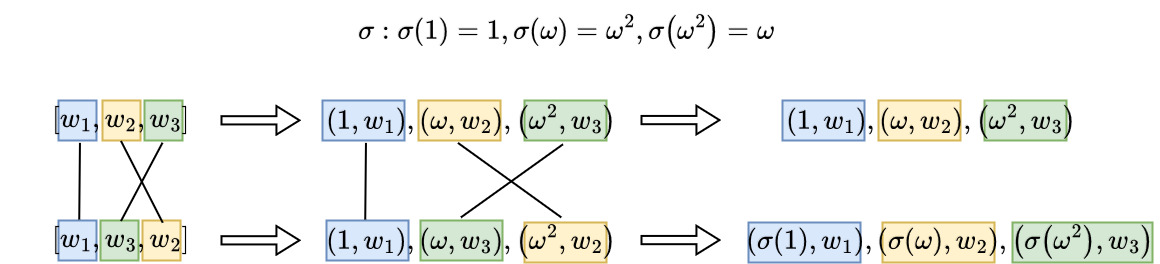
\includegraphics[width=1\linewidth]{round-figures/round2/tuple_encoding.jpg}
    \caption{Enforcing specific permutation}
\end{figure}

So, we will be comparing tuples $(\omega^{i-1}, w_i)$ to ensure that the specified permutation was applied: $$[(1, w_1), (\omega, w_2) \ldots (\omega^{n-1}, w_n)] \stackrel{?}{=} [(\sigma(1), w_1), (\sigma(\omega), w_2) \ldots (\sigma(\omega^{n-1}), w_n)]$$

The general permutation check \ref{permutation-check} relied on the fact that we were comparing polynomials, so now we somehow need to write the tuples as polynomials. We will construct a linear combination evaluated at a random point, so $(\omega^{i-1}, w_1)$ will become $w_i + \beta \omega_{i-1}$ where $\beta$ is randomly sampled.


Why can we use this encoding?
To use this check safely in the protocol, we need to be sure that $$(a, b) = (a', b') \iff a + \beta b = a' + \beta b'$$

Once again, the answer is polynomials. Notice that $a + \beta b$ is a linear polynomial with coefficients $a, b$ evaluated at $\beta$, and so is $a' + \beta b'$ just with different coefficients. If the random linear combinations are equal, then with very high probability, the tuples will also be equal. Now, we put everything together and finalize the intra-vector check for a particular permutation.
\begin{align*}
    (w_1 + \beta 1 + \gamma) \ldots  (w_n + \beta \omega^{n-1}+ \gamma) &\stackrel{?}{=} (w_1 + \beta \sigma(1) + \gamma) \ldots (w_n + \beta \sigma(\omega^{n-1}) + \gamma) \\
    \prod_{i = 1}^n w_i + \beta \omega^{i-1}+ \gamma &\stackrel{?}{=} \prod_{i = 1}^n  w_i + \beta \sigma(\omega^{i-1}) + \gamma \\
\end{align*}
$$1 \stackrel{?}{=} \frac{\prod_{i = 1}^n w_i + \beta \omega^{i-1}+ \gamma}{\prod_{i = 1}^n  w_i + \beta \sigma(\omega^{i-1}) + \gamma}$$
    

In summary, we have shown that the copy constraints of the arithmetic circuit could be represented as a permutation and found an effective way to ensure that these constraints are satisfied. Once again, the answer lay in converting everything to polynomials. The last obstacle in constructing the permutation polynomial is that we need to be able to check the permutation across multiple vectors.


\section{Inter-vector check}
In this case, we will want to check the permutation across vectors $w_l, w_r, w_o$, which are columns of the computation table described in \hyperref[chap:arithmetization]{arithmetization}. Each of $w_l, w_r, w_o$ has size $n$ and we will concatenate them into $$w = \{w_{l_1}, \ldots,w_{l_n}, w_{r_1}, \ldots,w_{r_n}, w_{o_1}, \ldots,w_{o_n}\}$$ which will have size $3n$. Now that we have changed the vector size, the domain $H$ is no longer sufficient for indexing $w$ because it has size $n$. We will solve this by using $H' = H \cup (k_1H) \cup (k_2H)$, where $k_1, k_2 \in \field$ are chosen such that $H, k_1H, k_2H$ are distinct meaning $\forall p, q, r: \omega^p \neq \omega^q k_1 \neq \omega^r k_2$. The permutation function $\sigma^*$ will create mapping $[1, 2, \ldots, 3n] \rightarrow H'$ which means $i \rightarrow \omega^i, n+i \rightarrow k_1 \omega^i, 2n+i \rightarrow k_2 \omega^i$. This is the permutation function that we mentioned in the protocol setup and it also implements rotation on the equivalence classes. Now, using the same idea as before, we can extend the check to inter-vector cases. $$1 \stackrel{?}{=} \prod_{i=1}^{n} \frac{f(i)}{g(i)}$$

\begin{equation}
\label{eq:prem-func}
    f(i) = (w_{i} + \beta \omega^i + \gamma)(w_{n+i} + k_1\beta\omega^i  + \gamma)(w_{2n+i} + k_2\beta\omega^i+ \gamma)
\end{equation}

\begin{equation}
    g(i) = (w_{i} + \beta\sigma^*(i) + \gamma)(w_{n+i} + \beta\sigma^*(n+i) + \gamma)(w_{2n+i} + \beta\sigma^*(2n+i) + \gamma)
\end{equation}


 
This expression might be undefined when $g(i)$ is 0; however, it can be proven that this only happens with negligible probability. When it happens, the protocol is instructed to abort and repeat with other randomly sampled $\beta, \gamma$.


\section{The Permutation Polynomial}
Now, we know how to perform the permutation check, but we would like to convince the verifier that it is correct. We cannot give him the values to compute the check because he would discover $w$, which violates zero-knowledge, and the computation would also be too heavy for the verifier. We will solve this problem by constructing the permutation polynomial, which is defined as:

\begin{equation}
    z(x) = 
    \begin{cases} 
          1 & x = \omega^0 \\
          \prod_{j=1}^{i} \frac{f(j)}{g(j)} & x = \omega^i \text{ where } i \in \{1, 2, 3, \ldots, n-1\}
    \end{cases}
\end{equation}


The essential idea of the permutation check remains the same. We are taking the product of ratios, where the numerator represents the former set and the denominator represents the permuted set. If each of these ratios is 1, the copy constraints are satisfied. How do we construct this polynomial? We will proceed as usual and perform Lagrange interpolation with the evaluation domain $H$:
$$(\frac{f(1)}{g(1)}, \frac{f(1)f(2)}{g(1)g(2)}, \frac{f(1)f(2)f(3)}{g(1)g(2)g(3)}, \ldots, \prod_{i=1}^{j} \frac{f(i)}{g(i)})$$

That means the (almost final) permutation polynomial could be written as:
$$z'(x) = \sum_{i=1}^{n-1} L_{i}(x) \prod_{j=1}^i \frac{f(j)}{g(j)}$$

This polynomial satisfies just the condition for $x = \omega^i \text{ where } i \in \{1, \ldots n-1\}$ and to enforce that permutation polynomial evaluates to 1 on $\omega^0$ we add the Lagrange basis $L_0(x)$. To finish it up, just add blinding scalars, but this time, we will need a blinding polynomial of degree 2 because later, there will be two openings of $z(x)$. 

\begin{equation*}
    z(x) = (b_7x^2 +b_8x +b_9)Z_H(x) + L_0(x) + z'(x)
\end{equation*}

Now, the prover needs to convince the verifier that it evaluates to 1 over $H$. If we do not include any addition checks, the prover could interpolate the following polynomial $[(1, 1),(\omega, 1),(\omega^2, 1) \ldots (\omega^{n-1}, 1)]$.

\procedureblock[linenumbering]{$Round2_{\prover}$}{
    \beta = \mathcal{H}(transcript, 0), \gamma = \mathcal{H}(transcript, 1) \\
    \text{compute permutation polynomial } z(x) \\
    \pcreturn [z]_1
}


% ==============================================================================
% ===ROUND3=====================================================================
% ==============================================================================
\section{Round 3}
\label{chap:round3}

The prover needs to combine checks from the previous rounds as well as convince the prover that the permutation polynomial was computed as specified by the protocol. But that is not all. We also need to handle the problem with polynomials exceeding the degree bound $n$. 

% \begin{figure}[H]
%     \centering
%     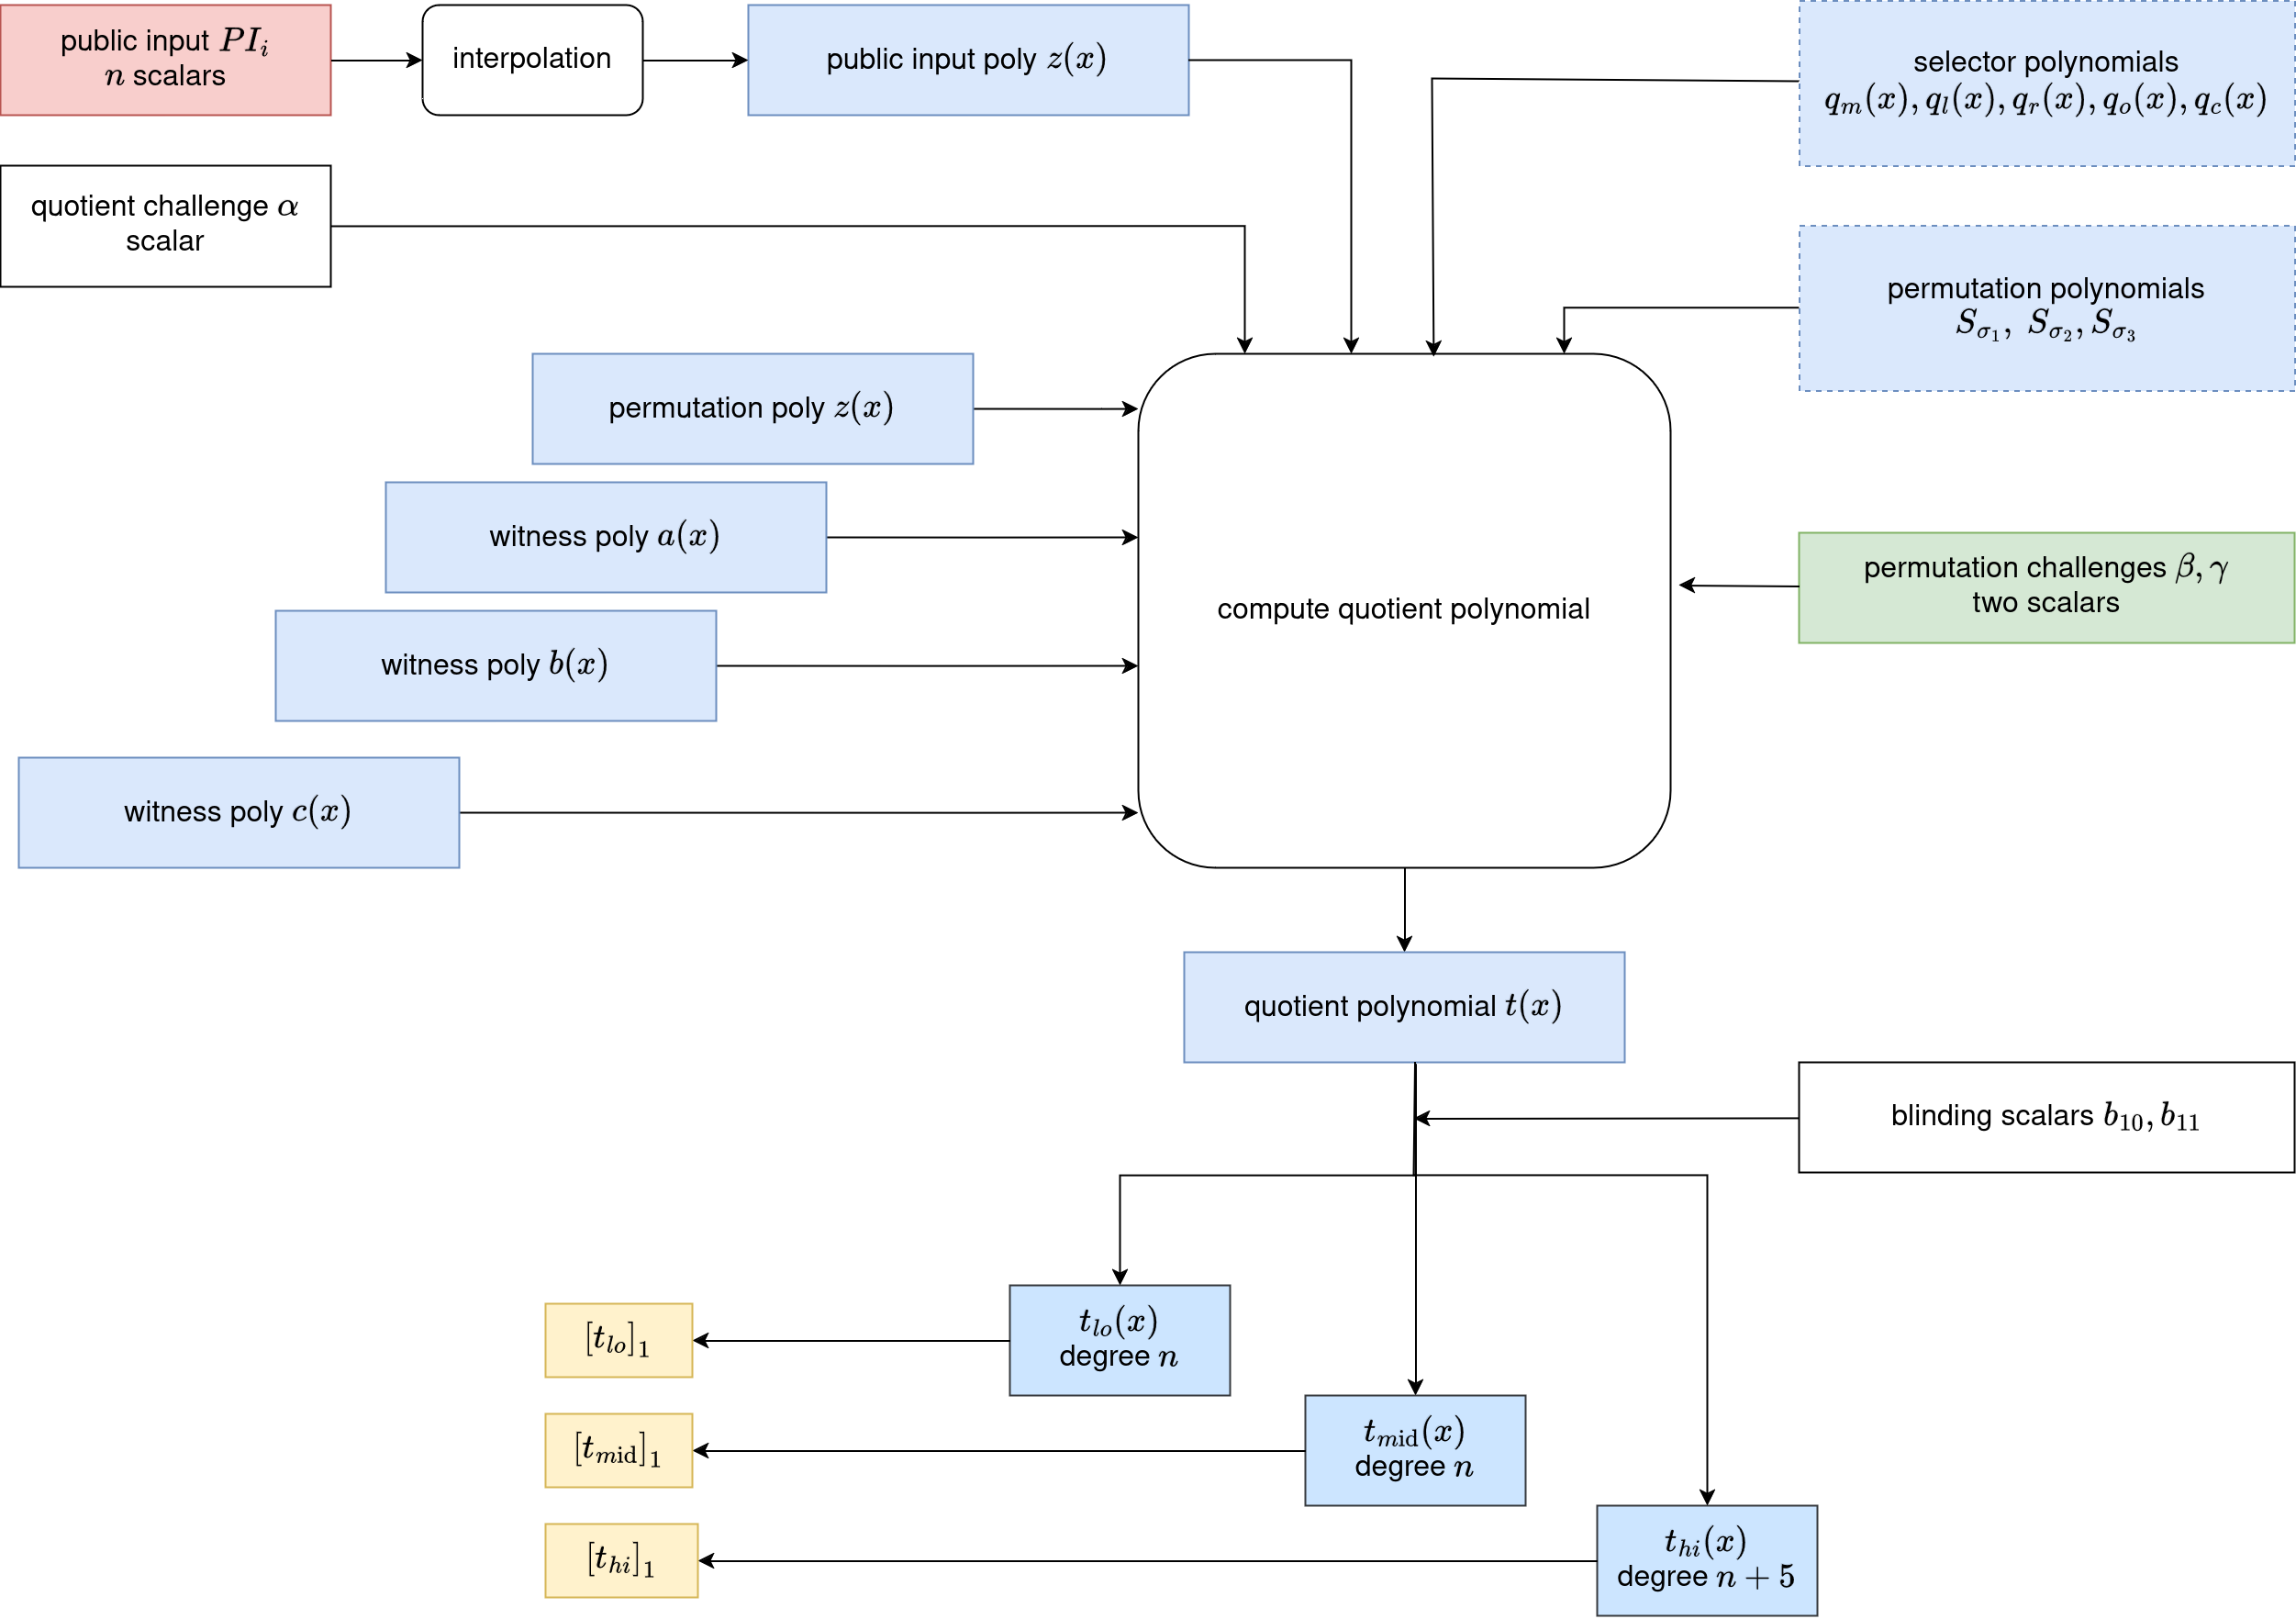
\includegraphics[width=1\linewidth]{round-figures/round3/round3.drawio.png}
%     \caption{Enter Caption}    
% \end{figure}


In the last round, we computed and committed to $z(x)$; however, we did not prove that it was computed correctly. Specifically we have promised that $z(\omega) = 1$, otherwise for $x = \omega^i$ it is cumulative product $\prod_{j=1}^i f(i) / g(i)$. This is the same as checking:

\begin{equation}
\label{eq:1-prem-check}
    (z(x)-1)L_0(x) = 0
\end{equation}
\begin{equation}
\label{eq:2-prem-check}
    z(x)\Tilde{f}(x) = \Tilde{g}(x)z(x\omega)
\end{equation}

$$\Tilde{f}(x) = (a(x) + x \beta + \gamma)(b(x) + x \beta k_1+ \gamma)(c(x) + x \beta k_2+ \gamma)$$
$$\Tilde{g}(x) = (a(x) + \beta S_{\sigma_1}(x) + \gamma)(b(x) + \beta S_{\sigma_2}(x)+ \gamma)(c(x) + \beta S_{\sigma_3}(x) + \gamma)$$

This is not immediately obvious. The proof is in \Cref{sec:computing-quotient-polynomial}. The quotient polynomial denoted as $t(x)$ in the paper consists of the sum of 3 expressions 
$t = t_1 + t_2 + t_3$:
\begin{equation}\label{quotient1}
    t_1(x) = (a(x)q_{l}(x) + b(x)q_{r}(x) + c(x)q_{o}(x) + a(x)b(x)q_{m}(x) + PI(x) + q_{c_i})\frac{1}{Z_H(x)}
\end{equation}

\begin{equation}\label{quotient2}
    t_2(x) = (f'(x)z(x))\frac{\alpha}{Z_H(X)} - (g'(x)z(\omega x))\frac{1}{Z_H(x)}
\end{equation}

\begin{equation}\label{quotient3}
    t_3(x) = (z(x)-1)L_1(x\frac{1}{Z_H(x)}
\end{equation}

$$t(x) = t_1(x) + t_2(x) \alpha + t_3(x) \alpha^2$$

The quotient polynomial might be long but comprises elements that make sense. So let's work through it.

\subsection{Computing quotient polynomial}
\label{sec:computing-quotient-polynomial}

\subsubsection{3rd term}
This corresponds to checking the first part of the $z(x)$ definition. So let's prove it is correct: 
\begin{lemma}[First property of permutation polynomial]
    $\forall x \in H: (z(x)-1)L_1(x) = 0 \implies z(\omega) = 1$
\end{lemma}

\begin{proof}
    For $x \neq \omega$, the Lagrange basis evaluates to 0, and there is no constraint for $z(x)$. However for $x = \omega$ we get $z(\omega) - 1 = 0$ meaning that $z(\omega)$ indeed must be equal to 1.
\end{proof}

\subsubsection{2nd term}
\begin{theorem}[First property of permutation polynomial]
    $\forall i \in [n]: z(\omega^i)f'(\omega^i) = g'(\omega^i)z(\omega^{i+1}) \implies \forall i \in [n]: z(\omega^i) = \prod_{j=1}^{i-1} \frac{f'(\omega^j)}{g'(\omega^j)}$
\end{theorem}

\begin{lemma}
    We will show this by induction. For the base case $i=1$ we get:
    $$z(\omega)f(\omega) = g(\omega)z(\omega^2)$$
    $$z(\omega^2) = \frac{f(\omega)}{g(\omega)}$$
    We know that $z(\omega) = 1$ is already checked for that; the rest simplifies easily. For the case $i =k+1$
    $$z(\omega^{k+1})f(\omega^{k+1}) = g(\omega^{k+1})z(\omega^{k+2})$$
    $$\prod_{j=1}^k \frac{f(\omega^j)}{g(\omega^j)} f(\omega^{k+1}) = g(\omega^{k+1})z(\omega^{k+2})$$
    $$\prod_{j=1}^k \frac{f(\omega^j)}{g(\omega^j)} \frac{f(\omega^{k+1})}{g(\omega^{k+1})} = z(\omega^{k+2})$$
    $$z(\omega^{k+2}) = \prod_{j=1}^{k+1} \frac{f(\omega^j)}{g(\omega^j)}$$    
\end{lemma}


\subsubsection{1st term}
These are the gate constraints introduced in the overview \eqref{chap:arithmetization}. Including them in the quotient polynomial makes sure they hold for each gate. 

Each check passes if the designated polynomial is zero on the evaluation domain. We want to combine to batch these checks such that $t(x) = 0 \iff t_1(x) = 0 \wedge t_2(x) = 0 \wedge t_3(x) = 0$. To achieve this, we will construct the quotient polynomial using random challenge $\alpha$:
$$t(x) = t_1(x) + t_2(x)\alpha + t_3(x)\alpha^2$$.

This technique is standard for batching checks in cryptography. The intuition on why this approach is secure is that the challenge is determined by the transcript, which contains the commitments to the polynomials that construct $t(x)$. So, the prover cannot make assumptions about the challenge before the commitment.

\subsection{Splitting quotient polynomial}
\label{sec:polynomial-splitting}

We can finally construct the quotient polynomial $t(x)$. However, the problem is that the polynomial degree is too big. We want our polynomials to have the maximum degree of $n$ to be able to commit to them. While creating SRS, we assumed so in the setup, and the whole KZG commitment scheme relies on it. We can split $t(x)$ into $< n$ degree polynomials $t_{lo}'(x), t_{mid}'(x)$ and $t_{hi}'(x)$ of degree at most $n+5$ such that: $$t(x) = t_{lo}'(x) + x^nt_{mid}'(x) + x^{2n}t_{hi}'(x)$$.

Why $t_{hi}$ has degree bound $n+5$? The degree of $t(x)$ is determined by $t_2(x)$ where we multiply wire polynomials $a(x), b(x), c(x)$ and permutation polynomial $z(x)$. Each of the wire polynomials has degree bound $n+1$, and the permutation polynomial has $n+2$, which makes it $4n+5$, but $t_2(x)$ is also divided by $Z_H(x)$ of degree $n$. Therefore the degree bound of the quotient polynomial $t(x)$ is $3n+5$. This means $t(x)$ can be written as $t(x) = c_0 + c_1x \ldots c_{3n+5}x^{3n+5}$. Then we can split as:
$$t'_{lo}(x) = c_0 + c_1 x + c_2 x^2 \ldots c_{n-1}x^{n-1}$$
$$t'_{mid}(x) = \frac{c_{n}x^{n} + c_{n+1}x^{n+1} \ldots c_{2n-1}x^{2n-1}}{x^n}$$
$$t'_{hi}(x) = \frac{c_{2n}x^{2n} + c_{2n+1}x^{2n+1} \ldots c_{3n-5}x^{3n-5}}{x^{2n}}$$

Blinding with $b_{10}, b_{11} \in \field$ is performed as follows: $t_{lo}(x) = t_{lo}'(x) + b_{10}x^n , t_{mid}(x) = t_{mid}'(x) - b_{10} + b_{11}x^n, t_{hi}(x) = t_{hi}'(x) - b_{11}$. Now we are ready to calculate commitments with a degree at most $n+5$: $[t_{lo}(s)]_1, [t_{mid}(s)]_1, [t_{hi}(s)]_1$.

\procedureblock[linenumbering]{$Round3_{\prover}$}{
    \alpha \gets \field \\
    t(x) =  t_1(x) + t_2(x) \alpha + t_3(x) \alpha^2 \\
    t(x) -> t_{lo}, t_{mid}, t_{high} \\
    \pcreturn [t_{lo}]_1, [t_{mid}]_1, [t_{high}]_1
}

% ==============================================================================
% ===ROUND4=====================================================================
% ==============================================================================
\section{Round 4}
\label{chap:round4}

% \begin{figure}[H]
%     \centering
%     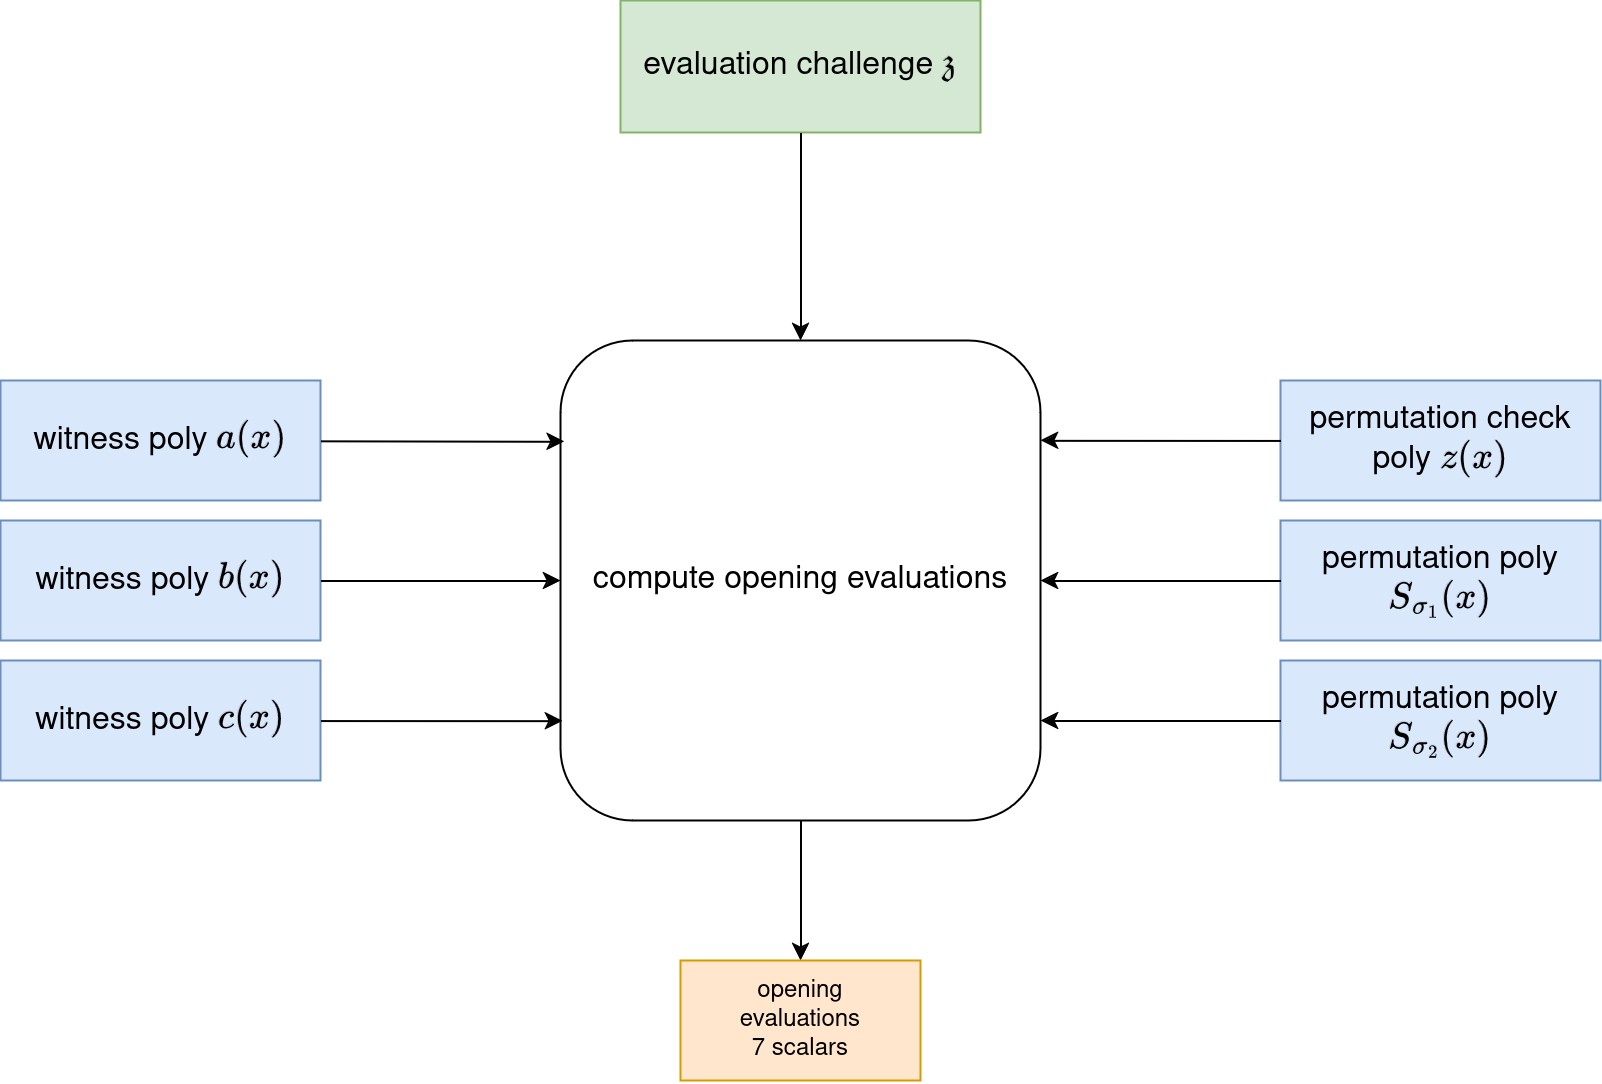
\includegraphics[width=1\linewidth]{round-figures/round4/round4.drawio.png}
%     \caption{Enter Caption}
    
% \end{figure}

In this round, the prover computes evaluation openings, denoted with a horizontal line above. The openings are performed at a random point $\challenge$. In an interactive case, $\challenge$ is chosen by the verifier; it is given by a hash function applied to a transcript of the prover computation. All the prover has to do is calculate and output: $\overline{a} = a(\challenge), \overline{b} = b(\challenge), \overline{c} = c(\challenge), \overline{z_\omega} = z(\omega\challenge),\overline{S}_{\sigma_1} = S_{\sigma_1}(\challenge), \overline{S}_{\sigma_2} = S_{\sigma_2}(\challenge)$. It is as simple as that. Now, let's look at ways to minimize the number of openings to reduce protocol communication costs.

\subsection{Linearization trick}
Imagine that the prover wants to show that $h_1(x)h_2(x) - h_3(c) = 0$ over a specified domain. Then he sure needs to commit to these polynomials and send their openings at a random $\challenge$, resulting in 3 commitments and three openings. Verifier needs to check $\forall x \in H: h_1(x)h_2(x) - h_3(c) = 0$ which thanks to \href{https://en.wikipedia.org/wiki/Schwartz%E2%80%93Zippel_lemma}{Schwartz-Zippel} simplifies to checking just at a single random point $\challenge$. 

\pseudocodeblock[head=Standard approach]{
    \text{Prover } \prover \< \< \text{Verifer } \verifier \\
    \< \< \\[-0.5 \baselineskip]
    f_1(x), f_2(x), f_3(x) \< \< \< \\
    \text{get challenge } \challenge \< \< \< \\
    \overline{f_1}, \overline{f_2}, \overline{f_3}  \< \< \< \\
    \< \sendmessageright*{\relax[f_1]_1, [f_2]_1, [f_3]_1} \< \\
    \< \sendmessageright*{\overline{f_1}, \overline{f_2}, \overline{f_3}} \< \\
    \< \< \text{verify openings} \\
    \< \< \overline{f_1} \overline{f_2} + \overline{f_3} \stackrel{?}{=} 0 \\
}

There is a better approach where the prover sends 3 commitments but just two 2 openings. This minimizes both the communication load and the proof size. The trick is in constructing a linearization polynomial: $l(x) = \overline{f_1} f_2(x) - f_3(x)$. As before the prover needs to send commitments $[f_1]_1, [f_2]_1, [f_3]_1$, but the openings are $\overline{f_1} = f_1(\mathfrak{z})$ and $\overline{l} = l(\mathfrak{z}) = \overline{f_1}\overline{f_2} - \overline{f_3}$.

Why is the prover not sending commitment to the linearization polynomial $l(x)$? Simply because the verifier can calculate $[l]_1$ on his own. Revise commitments are defined as $[f]_1 = G_1^{f(\tau)}$ elements of a group defined by points on an elliptic curve over a finite field $\mathbb{F}_p$. In the group, only one operation is defined between the group elements: addition. This means that we can add commitments but not multiply them. However, it is possible to multiply a group element by a constant so we can calculate $[l]_1 = \overline{f_1}[f_2]_1 - [f_3]_1$. This means that to calculate commitment to the linearization polynomial, there can be only the addition of polynomials but not multiplication. 

So, if the prover can reconstruct commitment to the linearization polynomial $[l]_1$, he is also able to check that the opening $\overline{l}$ is a correct evaluation at $\mathfrak{z}$. Since the linearization polynomial is constructed as $l(x) = \overline{f_1}f_2(x) - f_3(x)$ it means checking $\overline{l} \stackrel{?}{=}$ is equivalent to checking $\overline{f_1}\overline{f_2} - \overline{f_3} \stackrel{?}{=} 0$.


\pseudocodeblock[head=Linearization trick]{
    \text{Prover } \prover \< \< \text{Verifer } \verifier \\
    \< \< \\[-0.5 \baselineskip]
    f_1(x), f_2(x), f_3(x) \< \< \< \\
    \text{get challenge } \challenge \< \< \< \\
    l(x) = \overline{f_1} f_2(x) + f_3(x)  \< \< \< \\
    \< \sendmessageright*{\relax[f_1]_1, [f_2]_1, [f_3]_1} \< \\
    \< \sendmessageright*{\overline{l}, \overline{f_1}} \< \\
    \< \< [l]_1 = \overline{f_1}[f_2]_1 + [f_3]_1 \\
    \< \< \text{verify openings} \\
    \< \< \overline{l} \stackrel{?}{=} 0 \\
}

Why is it not possible to use the curve pairings? We have defined curve pairing as a mapping $e: \mathbb{G}_1 \times \mathbb{G}_2 \rightarrow \mathbb{G}_t$. So, it is possible to perform "multiplication" of two group elements and end up in another target group. In the context of KZG, the verifier performs the check in the target group as $$e(C G_1^{-v}, G_2) \stackrel{?}{=} e(W, G_2^{\tau}G_2^{-z})$$. Very informally, this "multiplication" can be performed only once. After the multiplication, we end up with points in the target group where we cannot perform another multiplication unless we have some different mapping. So, a very high-level explanation for why we do not use the curve pairings in the linearization trick is that the pairing can be used only once in the protocol, and we reserve this for the verifier to do the KZG verification.


\procedureblock[linenumbering]{$Round4_{\prover}$}{
    \challenge = \mathcal{H}(transcript) \\
    \overline{a} = a(\challenge), \overline{b} = b(\challenge), \overline{c} = c(\challenge), \overline{z_\omega} = z_\omega(x), \overline{S}_{\sigma_1} = S_{\sigma_1}(x), \overline{S}_{\sigma_2} = S_{\sigma_2}(x) \\
    \pcreturn \overline{z_\omega}, \overline{S}_{\sigma_1}, \overline{S}_{\sigma_2}
}

% ==============================================================================
% ===ROUND5=====================================================================
% ==============================================================================
\section{Round 5}
\label{chap:round5}

% \begin{figure}[H]
%     \centering
%     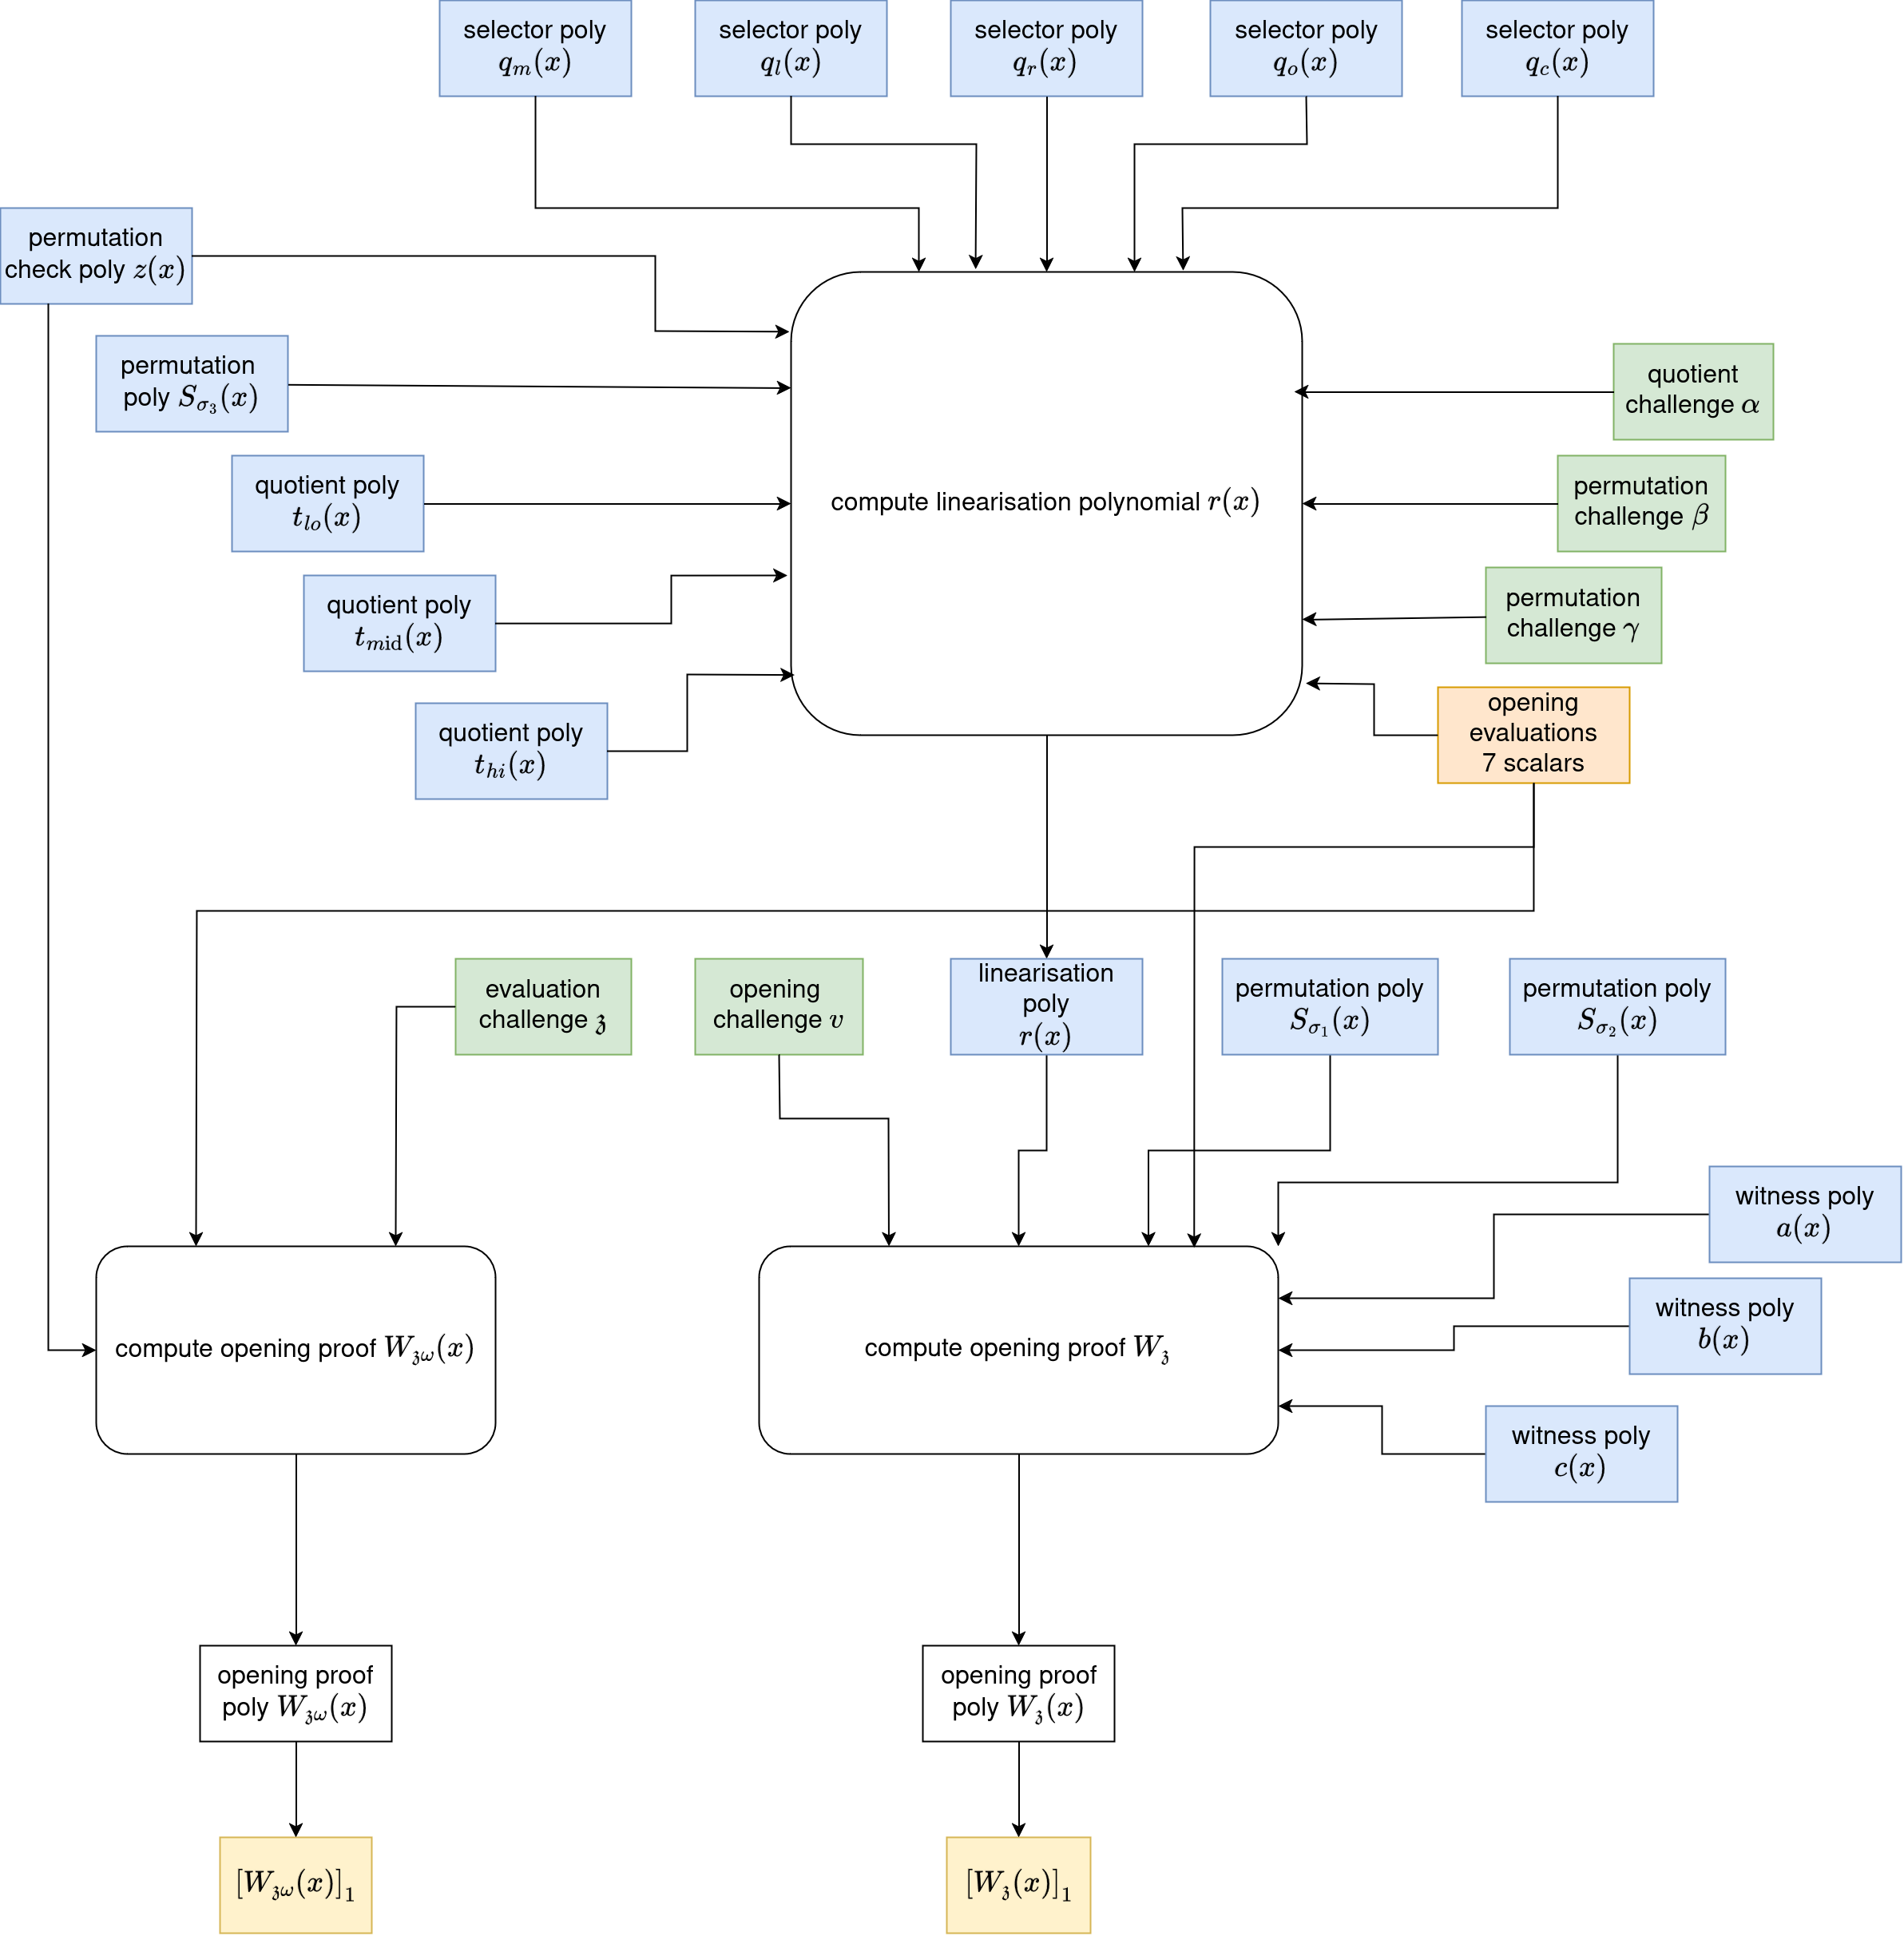
\includegraphics[width=1\linewidth]{round-figures/round5/round5.drawio.png}
%     \caption{Enter Caption}    
% \end{figure}

\subsection{Linearisation polynomial}
Recall from the \hyperref[chap:round3]{third round} that the quotient polynomial $t(x)$ was split into 3 parts to reduce the degree. So it must hold: $$t_{lo} + x^{n}t_{mid}(x) + x^{2n}t_{hi} = \frac{t_1(x) + \alpha t_2(x) + \alpha^2t_3(x)}{Z_H(x)} = t(x)$$

This means that over the whole evaluation domain $H$, it should hold that: 
\begin{equation}
    \label{linearization-base}
    0 = t_1(x) + \alpha t_2(x) + \alpha^2 t_3(x) - Z_H(x)(t_{lo} + x^{n}t_{mid}(x) + x^{2n}t_{hi})
\end{equation}

This is the base of how we will construct the linearisation polynomial $r(x)$. Some of the terms in $t_1(x), t_2(x), t_3(x)$ are substituted with the openings $\overline{a}, \overline{b}, \overline{c}, \overline{z_\omega}, \overline{S}_{\sigma_1}, \overline{S}_{\sigma_2}$ calculated in \hyperref[chap:round4]{round 4}. The linearisation polynomial can be written as:
\begin{align*}
    r(x) = &\overline{a}\overline{b}q_m(x) + \overline{a}q_l(x) + \overline{b}q_r(x) + \overline{c}q_o(x) + PI(\challenge) + q_c(x) \\
           &+\alpha [(\overline{a} + \beta \challenge + \gamma)(\overline{b} + \beta k_1 \challenge + \gamma)(\overline{c} + \beta k_2 \challenge + \gamma)z(x) \\
           &-(\overline{a} + \beta \overline{s}_{\sigma_1} + \gamma)(\overline{b} + \beta \overline{s}_{\sigma_2} + \gamma)(\overline{c} + \beta S_{\sigma_3}(x) + \gamma)\overline{z}_{\omega}] \\
           &+\alpha^2 [(z(x) -1)L_0(\challenge)] \\
           &-Z_H(\challenge)(t_{lo}(x) + \challenge^n t_{mid}(x) + \challenge^{2n} t_{hi}(x))
\end{align*}

The whole polynomial corresponds to the quotient polynomial minus $Z_H(\challenge)(t_{lo}(x) + \challenge^n t_{mid}(x) + \challenge^{2n} t_{hi}(x))$.
\begin{itemize}
    \item The first line represents the arithmetic gate check corresponding to the $t_1(x)$ \ref{quotient1} in the quotient polynomial $t(x)$. 
    \item Lines 2 and 3 represent the second check of the permutation polynomial \ref{eq:2-prem-check}, which is described by $t_2(x)$ in $t(x)$
    \item The line 4 is the first check of the permutation polynomial \ref{eq:1-prem-check}, which corresponds to $t_3(x)$ in $t(x)$
    \item The last line is from the expression above \ref{linearization-base}.
\end{itemize}

Since we "derived" the linearization polynomial from the expression \ref{linearization-base}, it should hold that $r(x)$ is zero over the whole domain $H$. Notice which polynomials are evaluated (denoted with the horizontal line). As described in the previous round, the linearization polynomial can contain polynomial additions and multiplication of polynomials by a constant, but not multiplication of two polynomials. And that is exactly what we are trying to achieve here. The openings are picked so that there is a single multiplication of polynomials. The terms $Z_H(\mathfrak{z}), L_0(\mathfrak{z})$ are in fact constants. This allows us to use the linearization trick, and as a result, the prover does not send the commitment $[r]_1$ because the verifier can calculate it independently. 

The big picture is that the prover is trying to prove: $0 = t_1(x) + \alpha t_2(x) + \alpha^2 t_3(x) - Z_H(x)(t_{lo} + x^{n}t_{mid}(x) + x^{2n}t_{hi})$. If he did it naively, he would need to send an opening to every single polynomial. However, thanks to the linearization trick, we are able to minimize the number of openings, thus also reducing the proof size.


\subsection{Opening proof polynomial}
The prover needs to send proof of opening for $\overline{a}, \overline{b}, \overline{c}, \overline{S}_{\sigma_1}, \overline{S}_{\sigma_2}$ at $\challenge$ and $\overline{z_\omega}$ at $\challenge\omega$. This is captured by the the polynomials $W_{\challenge}(x), W_{\challenge\omega}(x)$.


\subsubsection{First opening proof polynomial}
The opening proof polynomial is constructed by batching opening proof polynomials from the KZG polynomial commitment scheme in \Cref{chap:kzg}. We have proof polynomials:
\begin{align*}
  \frac{r(x)}{x-\challenge} &\xrightarrow{\text{proves}} r(\challenge) = 0  & \frac{a(x) - \overline{a}}{x-\challenge} &\xrightarrow{\text{proves}} a(\challenge) = \overline{a} \\
  \frac{b(x) - \overline{b}}{x-\challenge} &\xrightarrow{\text{proves}} b(\challenge) = \overline{b}  & \frac{c(x) - \overline{c}}{x-\challenge} &\xrightarrow{\text{proves}} c(\challenge) = \overline{c} \\
  \frac{S_{\sigma_1}(x) - \overline{S}_{\sigma_1}}{x-\challenge} &\xrightarrow{\text{proves}} S_{\sigma_1}(\challenge) = \overline{S}_{\sigma_1}  & \frac{S_{\sigma_2}(x) - \overline{S}_{\sigma_2}}{x-\challenge} &\xrightarrow{\text{proves}} S_{\sigma_2}(\challenge) = \overline{S}_{\sigma_2} \\
\end{align*}

These are batched using random challenge $v \in \field$ given by $\mathcal{H}(transcript)$. 

$$W_{\challenge}(x) = \frac{1}{x - \challenge} \left(
\begin{aligned}
    &r(x)  \\
    &+ v(a(x) - \overline{a}) \\ 
    &+ v^2(b(x) - \overline{b}) \\ 
    &+ v^3(c(x) - \overline{c}) \\
    &+ v^4(S_{\sigma_1}(x) - \overline{S}_{\sigma_1}) \\ 
    &+ v^5(S_{\sigma_2}(x) - \overline{S}_{\sigma_2}) 
\end{aligned}
\right)$$


\subsubsection{Second opening proof polynomial}
Prover calculates $W_{\challenge\omega}(x)$. Recall that in the quotient polynomial $t(x)$, both $z(x), z(z\omega)$ appear. Thanks to the linearization trick in \eqref{chap:round4}, it is sufficient to compute $\overline{z_\omega}$. However, as $z(x)$ is opened at $\challenge\omega$ instead of $\challenge$, we need a separated opening polynomial $W_{\challenge\omega}(x)$, which is the final polynomial that the prover needs to calculate.

$$W_{\challenge\omega}(x) = \frac{z(x)-\overline{z}_{\omega}}{x - \challenge\omega}$$

This polynomial checks that $z(\challenge\omega) = \overline{z}_\omega$ in the same way as described for the opening polynomial $W_{\challenge}(x)$. Now the prover can finally send the whole proof:
$$\pi = ([a]_1, [b]_1, [c]_1, [z]_1, [t_{lo}]_1, [t_{mid}]_1, [t_{hi}]_1, [W_{\challenge}]_1, [W_{\omega\challenge}]_1, \overline{a}, \overline{b}, \overline{c}, \overline{z_\omega}, \overline{S}_{\sigma_1}, \overline{S}_{\sigma_2})$$

% \[W_{\challenge}(x)\]_1, \[W_{\challenge\omega}(x)\]_1  \\
\procedureblock[linenumbering]{$Round5_{\prover}$}{
    v = \mathcal{H}(transcript) \\
    \text{Compute linearisation polynomial } r(x) \\
    \text{Compute opening proof polynomial } W_{\challenge}(x) \\
    \text{Compute opening proof polynomial } W_{\challenge\omega}(x) \\
    \pcreturn \pi
}

\section{Verification}
\label{sec:verification}

The verification verifier has its own preprocessed input and performs multiple sanity checks on the proof. The interesting part is the batched verification of KZG. Essentially the prover needs to validate $W_{\challenge}(x), W_{\challenge\omega}(x)$. The polynomials can be written in a simplified way as $W_{\challenge}(x) = F(x) / (x - \challenge)$, $W_{\challenge\omega}(x) = E(x) / (x - \challenge\omega)$ and after some rearranging we get:
\begin{equation}
    xW_{\challenge}(x) = \challenge W_{\challenge}(x) + F(x)
\end{equation}
\begin{equation}
    \label{batch-equation}
    xW_{\challenge\omega}(x) = \challenge\omega W_{\challenge\omega}(x) + E(x)
\end{equation}

Now, we can batch the expressions as in \Cref{batch-equation}.
\begin{equation}
    x(W_{\challenge}(x) + uW_{\challenge\omega}(x)) = \challenge W_{\challenge}(x) + u\challenge\omega W_{\challenge\omega}(x) + F(x) + uE(x)
\end{equation}

In the last steps of the verification algorithm, the verifier calculates the commitments to $[E]_1, [F]_1$. The final step checks the above identity using batched KZG-style verification with commitments and pairings.


% \hl{edit this}
% Now to describe this on KZG. For simplicity we have two polynomials $q_1(x), q_2(x)$ with commitments $c_1, c_2$. This approach can be generalized to any number of polynomials. We would like to check $q_1(z_1) = v_1, q_2(z_2) = v_2$ which is equivalent to divisibility check $q_1(x) = \frac{w_1(x) - v_1}{x - z_1}, q_2(x) = \frac{w_2(x) - v_2}{x - z_2}$. We can rearrange these as:

% $$x q_1(x) = w_1(x) + q_1(x)z_1$$
% $$x q_2(x) = w_2(x) + q_2(x)z_2$$

% Combining these with the batch challenge $\alpha$:
% $$xq_1(x) + \alpha x q_2(x) = z_1q_1(x) + w_1(x) + \alpha z_2 q_2(x) + \alpha w_2(x)$$

% Multiply both sides by generator $g$:
% $$xq_1(x)g + \alpha x q_2(x)g = z_1q_1(x)g + w_1(x)g + \alpha z_2 q_2(x)g + \alpha w_2(x)g$$

% Now we evaluate the expression at $\tau$:
% $$x([q_1]_1 + \alpha [q_2]_1) = z_1[q_1]_1 + y_1 + \alpha z_2 [q_2]_1 + \alpha y_2$$

% $$e(x([q_1]_1 + \alpha [q_2]_1), g) = e(z_1[q_1]_1 + y_1 + \alpha z_2 [q_2]_1 + \alpha y_2, g)$$


% All of the checks are eventually condensed into the polynomials $W_{\challenge}(x)$ and $W_{\challenge\omega}(x)$. 


